% !TEX encoding = UTF-8 Unicode
% -*- coding: UTF-8; -*-
% vim: set fenc=utf-8

\chapter{Arquitetura ARMFUL}%
\label{chap:arquitetura-armful}

Nesse capítulo será apresentada a arquitetura \abbrev{ARMFUL}{Analysis of Raw Data from Multiple Files} ARMFUL (do inglês: Analysis of Raw Data from Multiple Files; em tradução livre: Análise de Dados Científicos de Múltiplos Arquivos), introduzida recentemente em~\cite{silva2016situ,silva2017raw} pelo laboratório de \abbrev{NACAD}{Núcleo Avançado de Computação de Alto Desempenho} Núcleo Avançado de Computação de Alto Desempenho (NACAD) da \abbrev{UFRJ}{Universidade Federal do Rio de Janeiro} UFRJ (Universidade Federal do Rio de Janeiro). Também será abordado o \textit{DfAnalyzer}, uma instância dessa arquitetura, implementada pelo mesmo laboratório.

\section{Visão geral}

A \textbf{arquitetura ARMFUL} tem suporte a extração de dados científicos e a técnicas de indexação com o propósito de permitir o acesso direto a qualquer elemento ou região específica do espaço do fluxo de dados de uma simulação científica. Essa flexibilidade existe graças a uma \textbf{arquitetura de componentes}, que utiliza um SGWfC como bancos de dados de proveniência de dados para proporcionar um caminho de acesso entre o fluxo de dados e os dados científicos. Na \autoref{fig:armful-architecture}, podemos visualizar como é feita a divisão em componentes da ARMFUL. Eles são os seguintes:

\begin{itemize}
    \item Extração de dados científicos;
    \item Indexação de dados científicos;
    \item Catálogo de dados científicos;
    \item Ingestão de dados de proveniência;
    \item Processamento de consultas.
\end{itemize}

% REVIEW: do...aos VS entre...e os

\begin{figure}[ht]
    \centering
    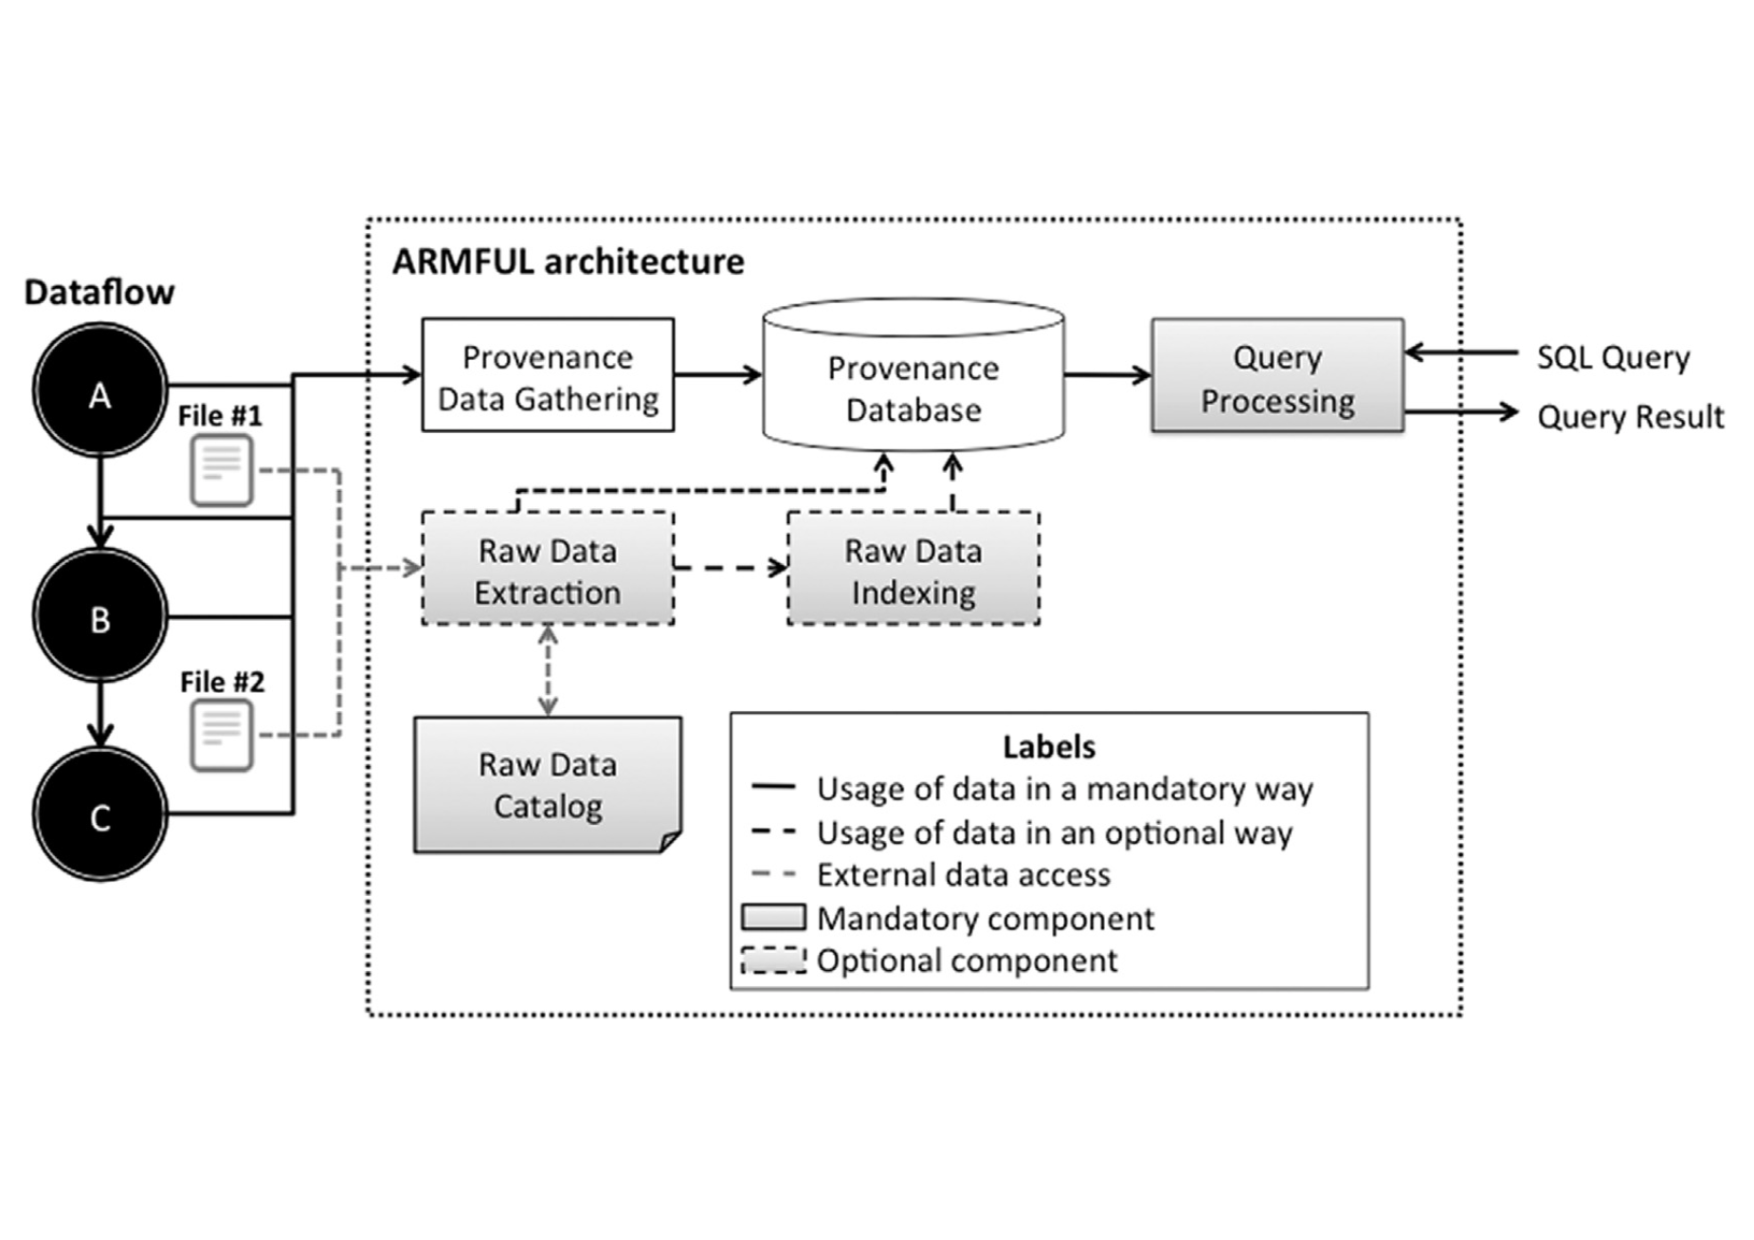
\includegraphics[width=\textwidth]{img/armful-architecture}
    \caption[Componentes da arquitetura ARMFUL]{Componentes da arquitetura ARMFUL. Encontrada originalmente em~\cite{silva2017raw}.}%
    \label{fig:armful-architecture}
\end{figure}

\perrotta{TODO: Expandir sobre o propósito da divisão em componentes, etc}

% DfAnalyzer (instância da ARMFUL) --> conjunto de componentes
% Provenance Gatherer (origem da proveniência para o banco de dados que eu vou utilizar na QueryProcessor)
% QueryProcessorCaptura de dados de proveniência}

\subsection{Extração e indexação de dados científicos}

% query tipo 1 --> in situ

% \subsection{Catálogo de dados científicos}

\subsection{Ingestão de dados}

% prov df (alimentar a base de dados com informacoes de proveniencia)
% ProvenanceGatherer

\subsection{Processamento de consultas}

% QueryProcessor

% melhor traduzir tudo, exceto DfAnalyzer

\section{DfAnalyzer: uma instanciação da arquitetura ARMFUL}

\subsection{Provenance Data Gatherer (PDG)}

\subsection{Raw Data Extractor (RDE)}

\subsection{Raw Data Indexer (RDI)}

% \subsection{Catálogo de dados científicos?}

\subsection{Query Processor (QP)}